\documentclass[12pt,a4paper]{article}
\usepackage{bold-extra}
\usepackage{appendix}
\usepackage{amsfonts,amsmath,amssymb}
\usepackage{enumerate}
\usepackage{float}
\usepackage{geometry}
\usepackage{graphicx}
\usepackage{latexsym}
\usepackage{listings}
\usepackage{multicol,multirow}
\usepackage{subfigure}
\usepackage{tabularx}
\usepackage{ulem}
\usepackage{tikz}
\usepackage{xcolor}
\geometry{a4paper,left=1in,right=1in,top=1in,bottom=1in}
\begin{document}
\centerline{\Huge{{\textbf{PHYSICS I\ \ Problem Set 7}}}}
\vspace{0.5cm}
\leftline{\large{Name: Haotian Fu}}
\rightline{\large{Student ID: 520021910012}}
\paragraph{\large \textbf{Problem 1}}~{\textbf{Solution}}
\vspace{2mm}\\
\noindent (a) 
\begin{align}
    F = \left( -\frac{\partial U}{\partial x}, -\frac{\partial U}{\partial y} \right) = (-y^2-2xy, -x^2-2xy)
\end{align}
\par Therefore, we can visialize it as
\begin{figure}[H]
    \centering
    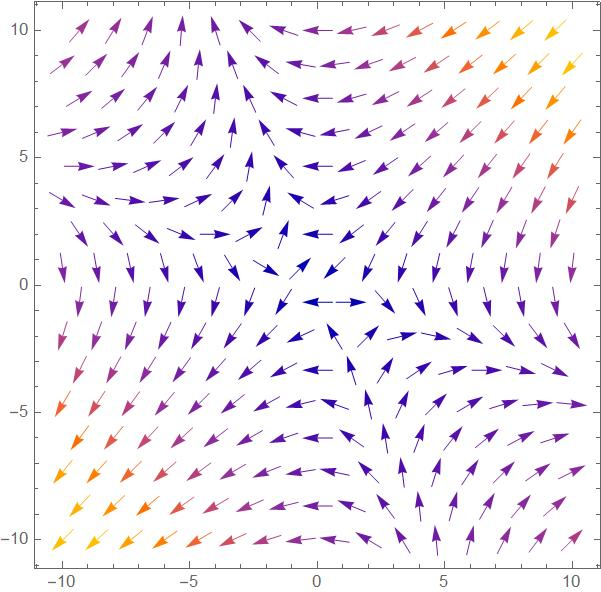
\includegraphics[width=0.3\linewidth]{1.jpg}
    \caption{Force in Problem 1}
    \label{fig-1}
\end{figure}
\noindent (b) 
\begin{figure}[H]
    \centering
    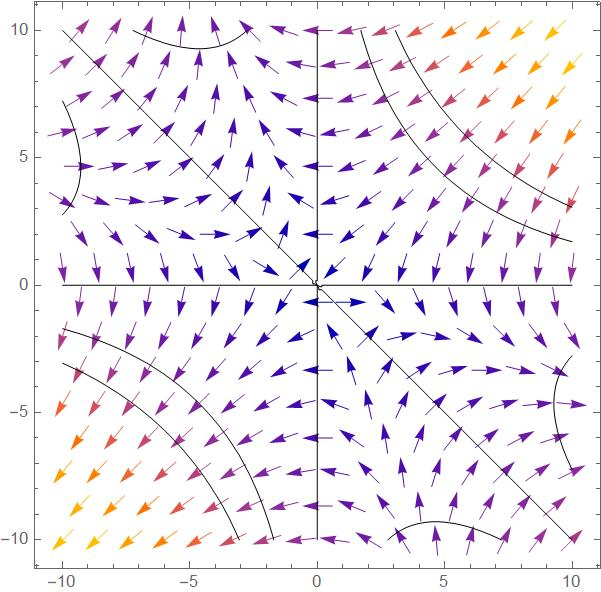
\includegraphics[width=0.3\linewidth]{2.jpg}
    \caption{Equipotential Diagram}
    \label{fig-2}
\end{figure}
\noindent (c) According to Fig 2, it is trivial that points are equipotential if $x=0$ or $y=0$ 
or $x=-y$ since all these circumstances the potential energy is equal to 0. Meanwhile, the other
curves all satisfy the equation $xy^2 + yx^2 = 0$.\\
\noindent (d) We decompose the displacemnet in $x-$axis and $y-$axis. Then we calculate the work 
along $x-$axis and $y-$axis separately. Suppose the trajectory is called $AB$.
\begin{align}
    W_x &= \int_{\Gamma_{AB}} F_x {\rm d} \bar{r}\\
    W_y &= \int_{\Gamma_{AB}} F_y {\rm d} \bar{r}\\
    \bar{r} &= \bar{x} + \bar{y}\\
    y &= x
\end{align}
\par Solving (1)(2)(3)(4)(5), we get
\begin{align}
    W = -2\quad [{\rm J}]
\end{align}
\noindent (e) Equation (5) changes into equation (7) due to the change of trajectory.
\begin{align}
    y = x^2
\end{align}
\par Solving (1)(2)(3)(4)(7), we get 
\begin{align}
    W = -2\quad [{\rm J}]
\end{align}

\paragraph{\large \textbf{Problem 2}}~{\textbf{Solution}}
\vspace{2mm}
\begin{figure}[H]
    \centering
    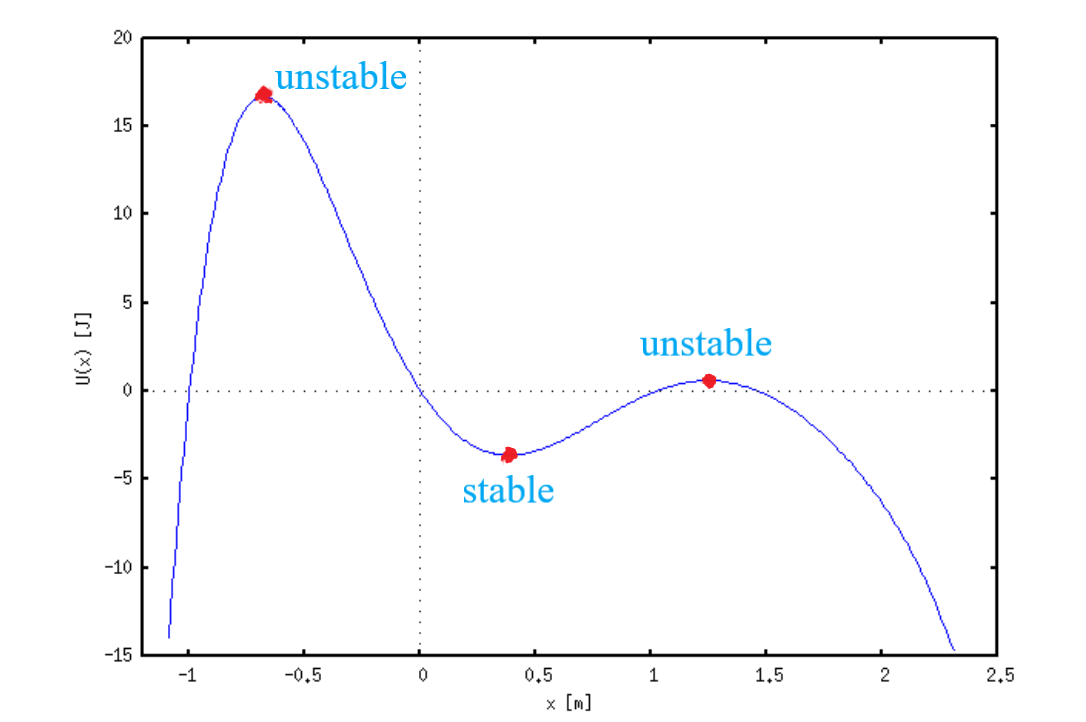
\includegraphics[width=0.7\linewidth]{1.png}
    \caption{Energy Diagram}
    \label{fig-3}
\end{figure}

\paragraph{\large \textbf{Problem 3}}~{\textbf{Solution}}
\vspace{2mm}\\
\noindent (a) Solving
\begin{align}
    F = -\frac{{\rm d}}{{\rm d}\bar{r}} U
\end{align}
\par we get 
\begin{align}
    F = 12U_0R_0^6\left( \frac{1}{r^{13}}\cdot R_0^6 - \frac{1}{r^7} \right)
\end{align}
\par Then we plot 
\begin{figure}[H]
    \centering
    \subfigure[Graph of U(r)]{
    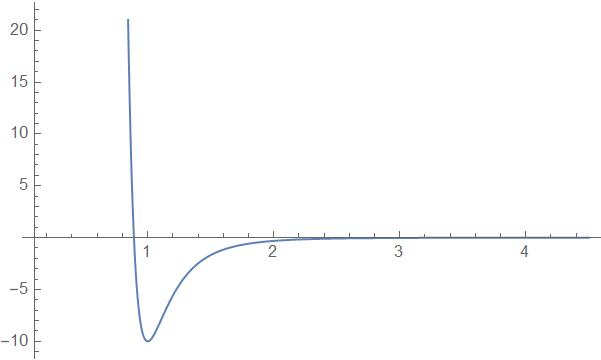
\includegraphics[width = 7cm]{3.jpg}
    }
    \subfigure[Graph pf F(r)]{
    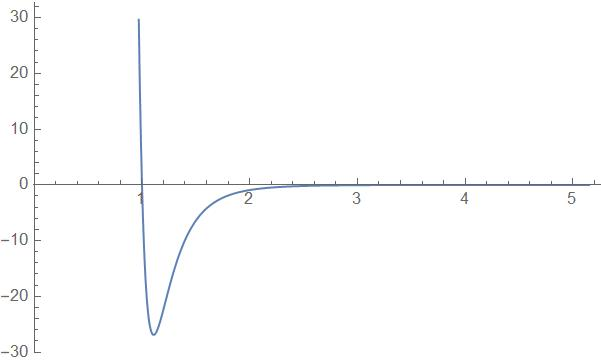
\includegraphics[width = 7cm]{4.jpg}
    }
    \caption{Graphs in Problem 3(a)}
\end{figure}
\par $12U_0R_0^{12}/r^{13}$ is responsible for repulsion while $-12U_0R_0^6/r^7$ is responsible for 
attraction.\\
\noindent (b) We rewrite the Lennard-Jones potential energy equation.
\begin{align}
    U = U_0\left( \left( \left( \frac{R_0}{r} \right)^6 - 1 \right)^2 - 1 \right)
\end{align}
\par Thus when $\left( \frac{R_0}{r} \right) = 1$, the potential energy reaches its minimum.
Namely, the whole system is at its equilibrium. Therefore, $R_0$ refers to the distance between
the pair of neutral atoms or molecules at equilibrium. Meanwhile, $U_0$ refers to the magnitude
of the lowest energy of the whole system.\\
\noindent (c) We may use harmonic approximation to address this problem. Since $r=R_0$ is the equilibrium
point
\begin{align}
    U(r) &\doteq U(R_0) + \frac{1}{2}\mathop{U}\limits^{\cdot\cdot} (R_0) (r-R_0)^2
\end{align}
\par Then
\begin{align}
    F(r) &= -\frac{{\rm d}U(r)}{{\rm d}r} = \mathop{U}\limits^{\cdot\cdot}(R_0) r -
    \mathop{U}\limits^{\cdot\cdot}(R_0) R_0 = \mathop{U}\limits^{\cdot\cdot}(R_0) (r - R_0)
\end{align}
\par For SHM
\begin{align}
    F(x) &= -kx\\
    \omega &= \sqrt{\frac{k}{m}}\\
    T &= \frac{2\pi}{\omega}
\end{align}
\par Solving (13)(14)(15)(16)
\begin{align}
    k &= \mathop{U}\limits^{\cdot\cdot}(R_0) = -\frac{72U_0}{R_0^2}\\
    T &= \frac{\pi}{3} \sqrt{\frac{mR_0^2}{2U_0}}
\end{align}
\noindent (d) The chemical interaction(like Van der Waals force) is oscillating here.

\paragraph{\large \textbf{Problem 4}}~{\textbf{Solution}}
\vspace{2mm}
\par The unit of $U_0$ is J while the unit of $\alpha$ is $\frac{1}{m}$
\par Suppose the equilibrium position is at $x_0$.
\begin{align}
    U(x) &\doteq U(x_0) + \frac{1}{2}\mathop{U}\limits^{\cdot\cdot} (x_0) (x-x_0)^2\\
    F(x) &= -\frac{{\rm d}}{{\rm d}x} U(x) = -\mathop{U}\limits^{\cdot\cdot}(x_0) (x-x_0)
\end{align}
\par Meanwhile
\begin{align}
    \mathop{U}\limits^{\cdot}(x) &= \frac{2U_0\alpha\sin\alpha x}{\cos^3\alpha x}\\
    \mathop{U}\limits^{\cdot}(x_0)&= 0\\
\Rightarrow\qquad x_0 &= 0
\end{align}
\par In addition
\begin{align}
    \mathop{U}\limits^{\cdot\cdot}(x) &= \frac{2\alpha^2U_0 + 4\alpha^2U_0\sin^2\alpha x}{\cos^4\alpha x}
\end{align}
\par Solving (23)(24)
\begin{align}
    \mathop{U}\limits^{\cdot\cdot}(x_0) &= 2\alpha^2U_0
\end{align}
\par For SHM
\begin{align}
    F &= -k(x-x_0)\\
    \omega &= \sqrt{\frac{k}{m}}\\
    T &= \frac{2\pi}{\omega}
\end{align}
\par Solving (20)(25)(26)(27)(28)
\begin{align}
    T = 2\pi \sqrt{\frac{m}{2\alpha^2U_0}}
\end{align}

\end{document}